%%%%%%%%%%%%%%%%%%%%%%%%%%%%%%%%%%%%%%%%%
% Beamer Presentation
% LaTeX Template
% Version 1.0 (10/11/12)
%
% This template has been downloaded from:
% http://www.LaTeXTemplates.com
%
% License:
% CC BY-NC-SA 3.0 (http://creativecommons.org/licenses/by-nc-sa/3.0/)
%
%%%%%%%%%%%%%%%%%%%%%%%%%%%%%%%%%%%%%%%%%

%----------------------------------------------------------------------------------------
%	PACKAGES AND THEMES
%----------------------------------------------------------------------------------------

\documentclass[14pt,handout]{beamer}
%%\documentclass[14pt]{beamer}

\mode<presentation> {

% The Beamer class slide themes
\usetheme{Madrid} %i was using this one

% Beamer class color themes

%\usecolortheme{albatross}

%\setbeamertemplate{footline} % To remove the footer line in all slides uncomment this line
%\setbeamertemplate{footline}[page number] % To replace the footer line in all slides with a simple slide count uncomment this line

%\setbeamertemplate{navigation symbols}{} % To remove the navigation symbols from the bottom of all slides uncomment this line
}

\usepackage{graphicx} % Allows including images
\usepackage{booktabs} % Allows the use of \toprule, \midrule and \bottomrule in tables
\usepackage{hyperref}
\usepackage{helvet}

%----------------------------------------------------------------------------------------
%	TITLE PAGE
%----------------------------------------------------------------------------------------

\title[SciWrite]{Scientific Writing} % The short title appears at the bottom of every slide, the full title is only on the title page

\author{C. Ryan Campbell} % Your name
\institute[Duke] % Your institution as it will appear on the bottom of every slide, may be shorthand to save space
{
Duke University \\ % Your institution for the title page
\medskip
\textit{c.ryan.campbell@duke.edu} % Your email address
}
\date{16 Nov 2017} % Date, can be changed to a custom date

\begin{document}

\begin{frame}
\titlepage % Print the title page as the first slide
\end{frame}


\begin{frame}
\frametitle{Overview} % Table of contents slide, comment this block out to remove it
\tableofcontents % Throughout your presentation, if you choose to use \section{} and \subsection{} commands, these will automatically be printed on this slide as an overview of your presentation
\end{frame}

%----------------------------------------------------------------------------------------
%	PRESENTATION SLIDES
%----------------------------------------------------------------------------------------

%------------------------------------------------
\section{Goals} 
%------------------------------------------------

%------------------------------------------------
\begin{frame}
\frametitle{Today's Goals}
%what students should know/learn today
\begin{itemize}
	\item<+-> Learn some guidelines for how to write a paper
	\item<+-> Ideas for how to apply those to the class project
	\item<+-> Generalize these to help write in other forms
\end{itemize}
\end{frame}

%------------------------------------------------
\begin{frame}
\frametitle{Review to Read}
\begin{itemize}
	\item<+-> This is a summary from:
	\item<+-> Mensh \& Kording. 2017.
\end{itemize}
\end{frame}

%------------------------------------------------
\begin{frame}
\frametitle{How does this apply to 490S?}
\begin{itemize}
	\item<+-> For each slide/segment we'll (try to) ask:
	\item<+-> What can we take from this for the project?
\end{itemize}
\end{frame}

%------------------------------------------------
\begin{frame}
\frametitle{How does this apply to life?}
\begin{itemize}
	\item<+-> What kinds of writing will you be doing?
	\item<+-> For each slide/segment we'll (try to) ask:
	\item<+-> What can we take from this for writing?
\end{itemize}
\end{frame}

%------------------------------------------------
\section{General Principles}
%------------------------------------------------

%------------------------------------------------
\begin{frame}
\frametitle{General Principles}
\begin{itemize}
	\item<+-> Focus on the Central Contribution
	\item<+-> Write for Humans Who Don't Know Your Work
	\item<+-> Context-Content-Conclusion
	\item<+-> Logical Flow - Parallelism
\end{itemize}
\end{frame}

%------------------------------------------------
\begin{frame}
\frametitle{Focus on the Central Contribution}
\begin{itemize}
	\item<+-> Measure success by the reader's comprehension and memory of the paper
	\item<+-> Can they repeat the main tenet back to you?
	\item<+-> Focus on this main tenet and build an argument around it
	\item<+-> Emphasize this tenet in the title
\end{itemize}
\end{frame}

%------------------------------------------------
\begin{frame}
\frametitle{Write for Humans Who Don't Know Your Work}
\begin{itemize}
	\item<+-> Very hard to analyze your own work as an outsider
	\item<+-> Think like a designer - each sentence should have a purpose
	\item<+-> People are easily distracted - tie points back to your main tenet
	\item<+-> Leaving loose points lying around will distract readers from the point
\end{itemize}
\end{frame}

%------------------------------------------------
\begin{frame}
\frametitle{Context-Content-Conclusion}
\begin{itemize}
	\item<+-> The beginning should set up the Context
	\item<+-> The middle should provide the Content
	\item<+-> The end should lead readers to your Conclusion
	\item<+-> Works best for research papers... how could other forms of writing differ?
\end{itemize}
\end{frame}

%------------------------------------------------
\begin{frame}
\frametitle{C-C-C Flowchart}
\begin{center}
	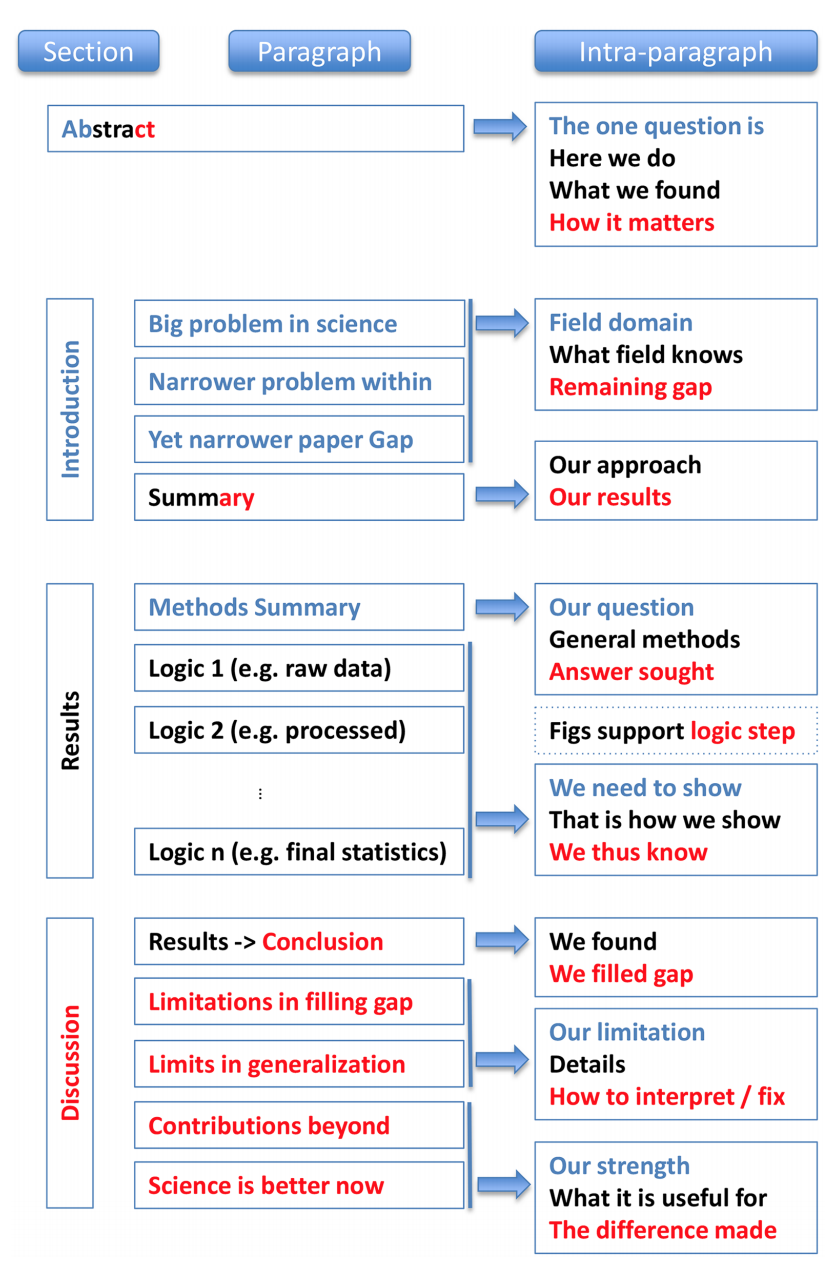
\includegraphics[width=.4\textwidth]{images_20171116_flowchart.png}
\end{center}
\end{frame}

%------------------------------------------------
\begin{frame}
\frametitle{Logical Flow - Avoid Zigzag}
\begin{itemize}
	\item<+-> Avoid ``Zig-zagging'' - bringing up topics and boucing to and fro
	\item<+-> The main tenet should be revisted often
	\item<+-> Other ideas and topics should be brought up to support the argument, then wrapped up
\end{itemize}
\end{frame}

%------------------------------------------------
\begin{frame}
\frametitle{Logical Flow - Parallelism}
\begin{itemize}
	\item<+-> Parallelism - communicate similar messages similarly, don't be afraid to repeat words or phrasing
	\item<+-> ``The gene patheway X shows higher expression in treated samples, providing support that this molecular machinery is integral to the cell's response to A''
	\item<+-> ``The gene patheway Y shows lower expression in treated samples, providing support that this molecular machinery is not integral to the cell's response to A''
	\item<+-> It may not seem poetic, but the repetition is helpful for the reader
\end{itemize}
\end{frame}

%------------------------------------------------
\begin{frame}
\frametitle{Logical Flow - Parallelism}
\begin{itemize}
	\item<+-> Changing words can be confusing
	\item<+-> ``The gene patheway X shows higher expression in treated samples, providing support that this molecular machinery is integral to the cell's response to A''
	\item<+-> ``The gene patheway Y measures lower expression in treated samples, lending support to the theory that this molecular machinery is not important to the cell's response to A''
\end{itemize}
\end{frame}

%------------------------------------------------
\section{Paper Components}
%------------------------------------------------

%------------------------------------------------
\begin{frame}
\frametitle{Paper Components}
\begin{itemize}
	\item<+-> Abstract = Complete Story
	\item<+-> Communicate Why It Matters in Intro
	\item<+-> Connect Results with Logical Flow
	\item<+-> Discuss How You Filled the Gap
\end{itemize}
\end{frame}

%------------------------------------------------
\begin{frame}
\frametitle{Abstract = Complete Story}
\begin{itemize}
	\item<+-> Many people only read the abstract, so make it good
	\item<+-> Question
	\item<+-> What we did
	\item<+-> What we found
	\item<+-> It matters because 
\end{itemize}
\end{frame}

%------------------------------------------------
\begin{frame}
\frametitle{C-C-C Flowchart}
\begin{center}
	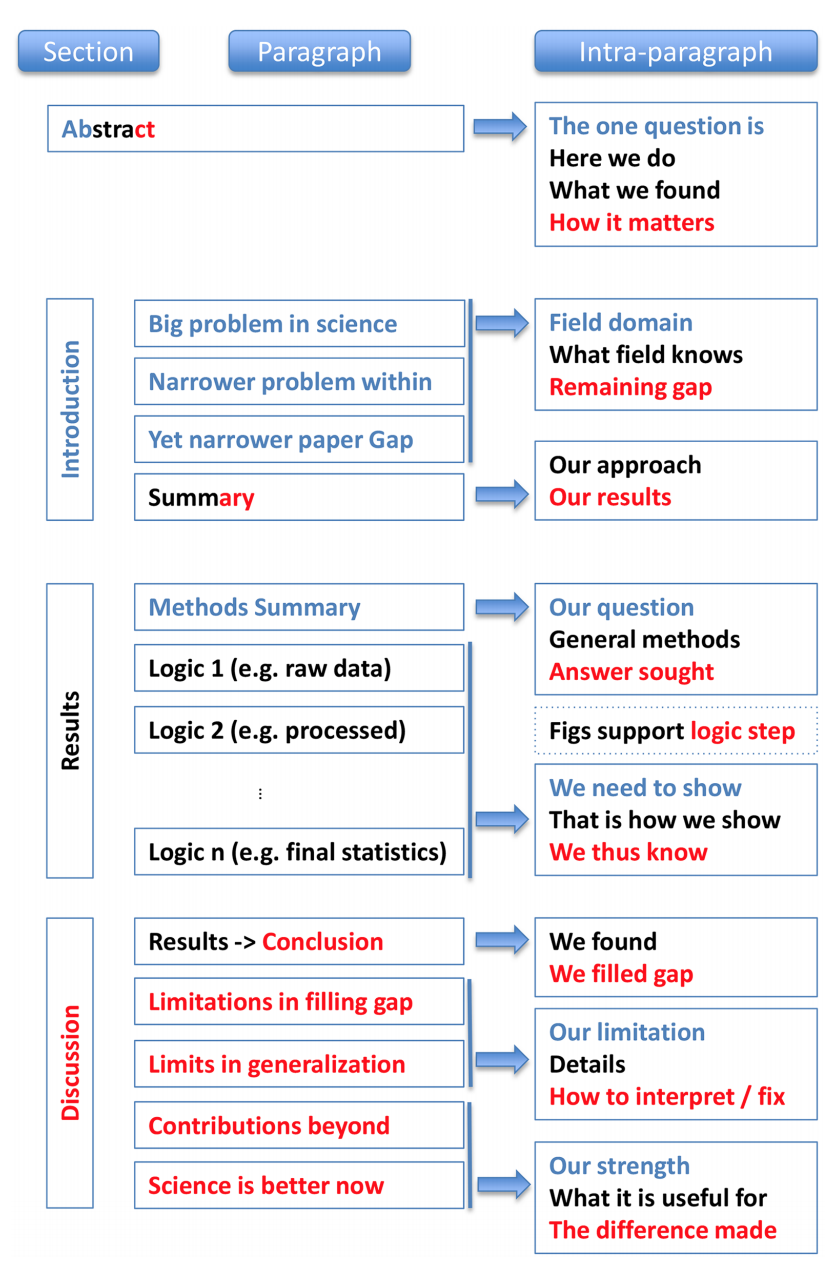
\includegraphics[width=.4\textwidth]{images_20171116_flowchart.png}
\end{center}
\end{frame}

%------------------------------------------------
\begin{frame}
\frametitle{Communicate Why It Matters in Intro}
\begin{itemize}
	\item<+-> Start broad (cliched, yes)
	\item<+-> Narrow while filling in current knowledge
	\item<+-> End with own study and results
\end{itemize}
\end{frame}

%------------------------------------------------
\begin{frame}
\frametitle{Connect Results with Logical Flow}
\begin{itemize}
	\item<+-> Each result is important to the overall tenet/idea
	\item<+-> Present each result in turn, with an brief intro sentence describing why it is crucial to the overall point
	\item<+-> ``To confirm that our sequencing was of good quality...''
	\item<+-> ``To verfiy that the sequenced reads were of the correct genome...''
	\item<+-> ``We tested the effect of condition on the cells...''
\end{itemize}
\end{frame}

%------------------------------------------------
\begin{frame}
\frametitle{Discuss How You Filled the Gap}
\begin{itemize}
	\item<+-> Describe the gap that was filled
	\item<+-> Mention limits to your finding
	\item<+-> Propose next steps to take down this scientific pathway
\end{itemize}
\end{frame}

%------------------------------------------------
\section{Process Tips}
%------------------------------------------------

%------------------------------------------------
\begin{frame}
\frametitle{Process Tips}
\begin{itemize}
	\item<+-> Put Time/Effort Where It Matters
	\item<+-> Get (and Implement) Feedback
\end{itemize}
\end{frame}

%------------------------------------------------
\begin{frame}
\frametitle{Put Time/Effort Where It Matters}
\begin{itemize}
	\item<+-> Title
	\item<+-> Abstract 
	\item<+-> Figures
	\item<+-> Overall outline
	\item<+-> How does this differ in other writing assignments?
\end{itemize}
\end{frame}

%------------------------------------------------
\begin{frame}
\frametitle{Get (and Implement) Feedback}
\begin{itemize}
	\item<+-> Writing is iterative optimization problem
	\item<+-> Re-read and re-edit many times
	\item<+-> Implementing changes can consist of scrapping a lot of what is there (not always just small edits)
	\item<+-> Important to take feedback from uninformed and informed readers
\end{itemize}
\end{frame}

%------------------------------------------------
\begin{frame}
\Huge{\centerline{The End}}
\end{frame}

%----------------------------------------------------------------------------------------

\end{document} 